\documentclass[t]{sdqbeamer}
%\documentclass[c]{sdqbeamer}

\usepackage{listings}
\usepackage{graphicx}
\usepackage{tabularx}
\usepackage{tikzsymbols}
\usepackage[lined,linesnumbered,ruled,noend]{algorithm2e}

\hypersetup{
	colorlinks=true,
	urlcolor=kit-orange
}

% set sdqbeamer options
\titleimage{blender-render}
\groupname{Algorithm Engineering}
\grouplogo{ae}
\selectlanguage{english}

% define title etc.pp.
\title[SAT Solving]{Practical SAT Solving}
\subtitle{Lecture 3}
\author{\underline{Markus Iser}, Dominik Schreiber, Tom\'a\v{s} Balyo}
\date{April 29, 2024}

% Existing KIT colors: kit-green, kit-blue, kit-red, kit-gray, kit-orange, kit-lightgreen, kit-brown, kit-purple, kit-cyan
% configure appearance
\setbeamercolor{block title}{bg=kit-blue}
\setbeamercolor{block body}{bg=kit-blue!10}
\setbeamercolor{block title example}{bg=kit-orange}
\setbeamercolor{block body example}{bg=kit-orange!10}
\setbeamertemplate{itemize item}{\color{kit-gray}\textbullet}
\setbeamertemplate{itemize subitem}{\color{kit-gray}\textbullet}
\setbeamercolor{item projected}{bg=kit-gray, fg=kit-gray}
\renewcommand{\insertnavigation}[1]{} % remove navigation bar

% define commands
\definecolor{myblue}{HTML}{0D3B66}
\definecolor{myred}{HTML}{6E0E0A}
\definecolor{mypink}{HTML}{F7B2B7}

\newcommand{\vars}[1]{\textsf{vars} (#1)}
\newcommand{\lits}[1]{\textsf{lits} (#1)}
\newcommand{\clss}[1]{\textsf{clss} (#1)}

\newcommand{\highl}[1]{\textcolor{myblue}{#1}}
\newcommand{\highlo}[1]{\textcolor{myred}{#1}}
\newcommand{\highlow}[1]{\textcolor{mypink}{#1}}

% Extra column types for tabularx
\newcolumntype{C}{>{\centering\arraybackslash}X}
\newcolumntype{L}{>{\raggedright\arraybackslash}X}
\newcolumntype{R}{>{\raggedleft\arraybackslash}X}

\newcommand{\setcolsep}[1]{\setlength{\tabcolsep}{#1}}
\newcommand{\setrowsep}[1]{\renewcommand{\arraystretch}{#1}}

% Definitions for the Tseitin transformation
\newcommand{\true}{\ensuremath{\mathit{True}}}
\newcommand{\false}{\ensuremath{\mathit{False}}}
\newcommand{\allvars}{\ensuremath{\mathcal{V}}}
\newcommand{\tseitin}[1]{\ensuremath{\mathcal{T}(#1)}}
\newcommand{\tseitinRec}[2]{\ensuremath{\mathcal{T}^{#2}(#1)}}
\newcommand{\tseitinSym}[1]{\ensuremath{\mathcal{T}_\mathsf{lit}(#1)}}
\newcommand{\tseitinDef}[2]{\ensuremath{\mathcal{T}_\mathsf{def}^{#2}(#1)}}
\newcommand{\hcancel}[2][black]{\setbox0=\hbox{$#2$}\rlap{\raisebox{.45\ht0}{\textcolor{#1}{\rule{\wd0}{1pt}}}}#2} 
\newcommand{\sateq}{\mathrel{\overset{\makebox[0pt]{\mbox{\normalfont\tiny\sffamily SAT}}}{=}}}

\newcommand{\enc}{\ensuremath{\mathcal{E}}} % encoding

% exercise commands
\newcommand{\exhead}[3]{
\hrule~\\[1ex]\noindent
{\bf Practical SAT Solving} (ST 2024) \hfill \fbox{Assignment #1} \\[1ex]
Markus Iser, Dominik Schreiber, Tom\'a\v{s} Balyo\\[1ex]
Algorithm Engineering (KIT) \hfill #2 -- #3\\
\hrule
\thispagestyle{empty}
}
\setlength{\itemsep}{1em}

\begin{document}

\begin{frame}
	\thispagestyle{empty}
	\titlepage
\end{frame}

\begin{frame}{Overview}
	\begin{block}{Recap. Lecture 2}
		\begin{itemize}\setlength{\itemsep}{1ex}
			\item Tractable Subclasses
			\item Constraint Encodings and their Properties
		\end{itemize}
	\end{block}
	\pause
	\begin{block}{Today's Topics: Elementary SAT Algorithms}
		\begin{itemize}\setlength{\itemsep}{1ex}
			\item Local Search
			\item Resolution
			\item DP Algorithm
			\item DPLL Algorithm
		\end{itemize}
	\end{block}
\end{frame}

\begin{frame}{Stochastic Local Search (SLS)}
\begin{block}{Minimize the Number of Unsatisfied Clauses}
	Start with a \highlo{random} complete variable assignment $\alpha$:
	\begin{center}
	  \resizebox*{0.8\textwidth}{!}{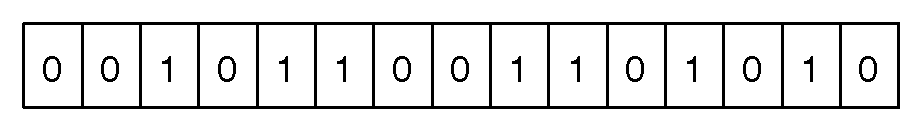
\includegraphics{figures/l03/random-ass-1.pdf}}
	\end{center}
	Repeatedly \highlo{flip} variables in $\alpha$ to decrease the number of unsatisfied clauses:
	\begin{center}
	  \resizebox*{0.8\textwidth}{!}{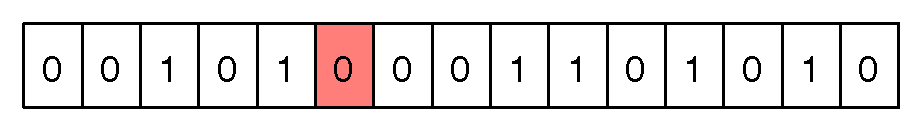
\includegraphics{figures/l03/random-ass-2.pdf}}
	\end{center}
\end{block}
\end{frame}
	
\begin{frame}{Stochastic Local Search (SLS)}
\begin{block}{Properties of SLS Algorithms}
	Local search algorithms are \highlo{incomplete}: They cannot show unsatisfiability!\\[1em]
	Challenges: 
	\begin{itemize}\setlength{\itemsep}{1ex}
		\item Which variable should be flipped next?
		\begin{itemize}\setlength{\itemsep}{1ex}
		\item<2-> select variable from an \highl{unsatisfied clause}
		\item<2-> select variable that \highl{maximizes} the number of satisfied clauses
		\end{itemize}
	\item<2-> How to avoid getting stuck in \highl{local minima}?
		\begin{itemize}\setlength{\itemsep}{1ex}
		\item<3-> randomization
		\end{itemize}
	\end{itemize}
\end{block}
\end{frame}
	
\begin{frame}{Classic SLS Algorithms}
\begin{block}{GSAT \href{http://dl.acm.org/citation.cfm?id=1867135.1867203}{(Selman et al., 1992)}}
\setlength\columnsep{1ex}
\begin{columns}[T]
	\begin{column}{.3\linewidth}
		~\\ Greedy local search algorithm
	\end{column}
	\begin{column}{.6\linewidth}
	\begin{algorithm}[H]
		\DontPrintSemicolon
		\caption{GSAT}
		\KwIn{ClauseSet $S$}
		\KwOut{Assignment $\alpha$, or Nothing}
		\BlankLine
		\For {$i = 1$ \KwTo MAX\_TRIES} {
			$\alpha$ = random-assignment to variables in $S$ \\
			\For {$j = 1$ \KwTo MAX\_FLIPS} {
				\lIf {$\alpha$ satisfies all clauses in $S$} {
					\Return $\alpha$
				}
				$x$ = variable that produces \highlo{least number of unsatisfied clauses} when flipped \\
				flip $x$
			}
		}
		\Return Nothing \tcp*{no solution found}
	\end{algorithm}
	\end{column}
\end{columns}
\end{block}
\end{frame}
	
\begin{frame}{SLS: Local Minima}
\begin{center}
	\only<1>{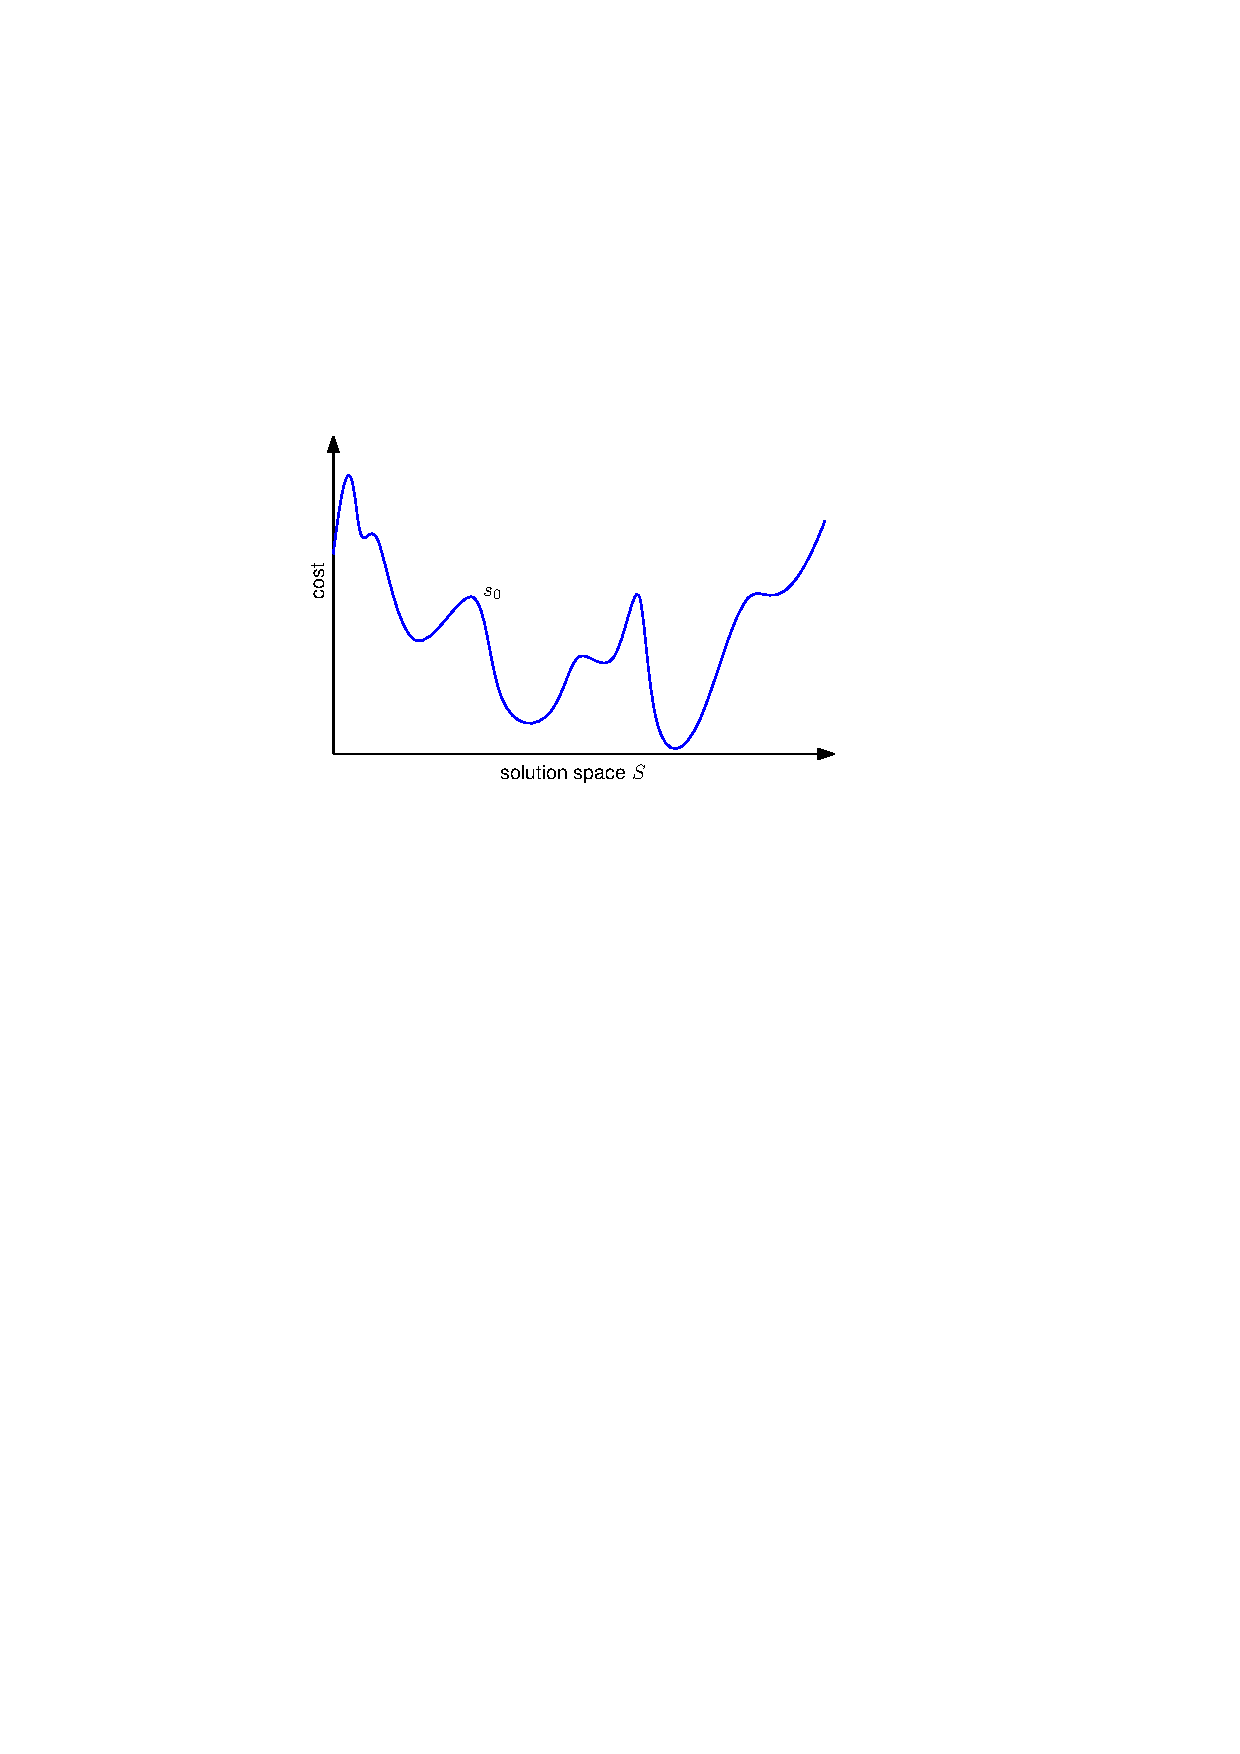
\includegraphics[width=0.56\textwidth,page=1]{figures/l03/sls-perturbation.pdf}}%
	\only<2>{\includegraphics[width=0.56\textwidth,page=2]{figures/l03/sls-perturbation.pdf}}%
	\only<3>{\includegraphics[width=0.56\textwidth,page=3]{figures/l03/sls-perturbation.pdf}}%
\end{center}
\begin{footnotesize}
\hfill [Illustration Adapted from: Alan Mackworth, UBC, Canada]
\end{footnotesize}
\end{frame}
	
\begin{frame}{Classic SLS Algorithms}
\begin{block}{WalkSAT \href{https://web2.qatar.cmu.edu/~gdicaro/15281/additional/dimacs93-walksat.pdf}{(Selman et al., 1993)}}
\setlength\columnsep{1ex}
\begin{columns}[T]
	\begin{column}{.3\linewidth}
		~\\ Variant of GSAT\\[1em]
		Try to avoid local minima by introducing \highl{random noise}.
	\end{column}
	\begin{column}{.6\linewidth}
	\begin{algorithm}[H]
		\DontPrintSemicolon
		\caption{WalkSAT($S$)}
		% \KwIn{ClauseSet $S$}
		% \KwOut{Assignment $\alpha$, or Nothing}
		% \BlankLine
		\For {$i = 1$ \KwTo MAX\_TRIES} {
			$\alpha$ = random-assignment to variables in $S$ \;
			\For {$j = 1$ \KwTo MAX\_FLIPS} {
				\lIf {$\alpha$ satisfies all clauses in $S$} {
					\Return $\alpha$
				}
				$C$ = \highl{random unsatisfied clause in $S$} \;
				\lIf {by flipping an $x \in C$ \highlo{no new unsatisfied clauses} emerges} {
					flip $x$
				}
				\lElse {
					\highl{with probability $p$ flip an $x \in C$ at random} \;
					otherwise, flip a variable that changes the \highlo{least number of clauses from satisfied to unsatisfied}
				}
			}
		}
		\Return Nothing \tcp*{no solution found}
	\end{algorithm}
	\end{column}
\end{columns}
\end{block}
\end{frame}
	
\begin{frame}{SLS: Important Notions}
\begin{block}{Consider a flip taking $\alpha$ to $\alpha'$}
	\begin{center}
	\setrowsep{1.5}
	\begin{tabularx}{\linewidth}{lX}
	\textbf{breakcount} & number of clauses \highl{satisfied} in $\alpha$, but \highlo{not satisfied in $\alpha'$} \\
	\textbf{makecount} & number of clauses \highlo{not satisfied} in $\alpha$, but \highl{satisfied in $\alpha'$} \\
	\textbf{diffscore} & \# unsatisfied clauses in $\alpha$ $-$ \# unsatisfied clauses in $\alpha'$ \\
	\end{tabularx}
	\end{center}
	Typically, {breakcount}, {makecount}, and/or {diffscore} are used to select the variable to flip.
\end{block}
\pause
\begin{block}{Recap using new nomenclature}
	\centering
	\setrowsep{1.5}
	\begin{tabularx}{\linewidth}{lX}
	\textbf{GSAT} & select variable with \highl{highest diffscore} \\
	\textbf{WalkSAT} & select variable with \highl{minimal breakcount} \\
	\end{tabularx}
\end{block}
\end{frame}
	
\begin{frame}{Stochastic Local Search (SLS)}
\begin{block}{Legacy of SLS}
\begin{itemize}\setlength{\itemsep}{1em}
	\item<1-> Extremely \highl{successful and popular} in early days of SAT
	\begin{itemize}\setlength{\itemsep}{1ex}
		\item SLS outperformed early resolution-based solvers, e.g., based on DP or DPLL
		\item for example, state of the art engine for \highl{automated planning} in the 90s
	\end{itemize}
	\item<2-> Today, sophisticated resolution-based systematic search solvers dominate in most practical applications
	\begin{itemize}\setlength{\itemsep}{1ex}
		\item Faster, more reliable, and \highlo{complete!}
	\end{itemize}
	\item<3-> Still useful as a component in more complex solvers
	\begin{itemize}\setlength{\itemsep}{1ex}
		\item Part of (parallel) \highl{algorithm portfolios}
		\item Control \highl{branching heuristics} in complete search algorithms
		\item Detection of autarkies in \highl{formula simplification} algorithms
		\item In combination with complete solvers for optimization problems (e.g., \highl{MaxSAT})
	\end{itemize}
\end{itemize}
\end{block}
\end{frame}

\begin{frame}{Recap}
\begin{block}{Elementary Algorithms}
	\begin{itemize}\setlength{\itemsep}{1em}
		\item Local Search
		\begin{itemize}\setlength{\itemsep}{1ex}
			\item Examples: GSAT, WalkSAT
			\item Terminology: breakcount, makecount, diffscore
		\end{itemize}
	\end{itemize}
\end{block}
\pause
\begin{block}{Next Up}
	\begin{itemize}\setlength{\itemsep}{1em}
		\item Resolution
	\end{itemize}
\end{block}
\end{frame}


\begin{frame}{Resolution}
\begin{block}{The Resolution Rule}
\vspace*{-3ex}
\begin{align*}
	\cfrac{P_1 \cup \{x\},\quad P_2 \cup \{\lnot x\}}{P_1 \cup P_2}
\end{align*}
Resolution is a logical \highlo{inference rule} to infer a \highlo{conclusion} (resolvent) from given \highlo{premises} (input clauses).
\end{block}
	
\begin{example}[Resolution]
\vspace*{-3ex}
\begin{align*}
	\{ \highlo{x_1}, x_3, \lnot {x_7} \}, \{ \highlo{\lnot {x_1}}, x_2 \} \quad &\vdash \quad \{ x_3, \lnot {x_7}, x_2 \} \\[1ex]
	\{ x_4, \highlo{x_5} \}, \{ \highlo{\lnot {x_5}} \} \quad &\vdash \quad \{ x_4 \} \tag{\highl{Fact}}\\[1ex]
	\{ \highlo{x_1}, \highlo{x_2} \}, \{ \highlo{\lnot {x_1}, \highlo{\lnot {x_2}}} \} \quad &\vdash \quad \{ x_1, \lnot {x_1} \} \tag{\highl{Tautological Resolvent}} \\[1ex]
	\{ \highlo{x_1} \}, \{ \highlo{\lnot {x_1}} \} \quad &\vdash \quad \{ \} \tag{\highl{Empty Clause}}
\end{align*}
\end{example}
\end{frame}
	
\begin{frame}{Resolution}
\begin{block}{Theorem: Resolution is Sound}
Given a CNF formula $F$ with two resolvable clauses $C_1, C_2 \subseteq F$ with resolvent $\operatorname{R}(C_1,C_2)$, the following holds:
\vspace*{-1ex}
\begin{align*}
	\highlo{F \quad \equiv~} \quad F \land \operatorname{R}(C_1,C_2)
\end{align*}
\end{block}
	
\begin{block}{Proof}
Let $C_1 := \{ x \} \cup P_1$ and $C_2 := \{ \lnot x \} \cup P_2$ such that $\operatorname{R}(C_1,C_2) = P_1 \cup P_2 =: D$.\\[1ex]

\textbf{Soundness:} $F \vdash F \land D \implies \highlo{F \models~} F \land D$ \\[.5ex]
Any satisfying assignment $\phi$ of $F$ is also a satisfying assignment of $D$:
Since $\phi$ satisfies both $C_1$ and $C_2$, it necessarily \highlo{satisfies at least one literal in $D$}. If $\phi$ satisfies $x$ then it satisfies some literal in $P_2$. Otherwise, if $\phi$ satisfies $\lnot x$ then it satisfies some literal in $P_1$.\\[1ex]
\pause
\textbf{Equivalence:} $F \vdash F \land D \implies F \land D \highlo{~\models F}$ \\[.5ex]
Since $D$ does not introduce new variables, $F \wedge D$ can not have more satisfying assignments than $F$.
\end{block}
\end{frame}
	
\begin{frame}{Resolution}
\begin{block}{Resolution is Sound and \highlow{Refutation} Complete}
\begin{itemize}\setlength{\itemsep}{1ex}
	\item If we manage to infer the \highlo{empty clause} from a CNF formula $F$, then $F$ is unsatisfiable. (sound)
	\item If $F$ is unsatisfiable, then there \highlo{exists a refutation by resolution}. (complete)
	\item \highlo{Not all possible} consequences of $F$ can be derived by resolution. (``only'' refutation complete)
\end{itemize}
\end{block}

\begin{block}{Resolution Proof}
A \highlo{resolution proof} for $F$ is a sequence of clauses $\langle C_1, C_2, \ldots, C_{k-1}, C_k = \emptyset \rangle$ where each $C_i$ is either an original clause of $F$ or a resolvent of two earlier clauses.
\end{block}

\begin{example}[Resolution Proof]
\vspace*{-3ex}
\begin{align*}
	F =& \{ x_1, x_2 \}, \{ \lnot x_1, x_2 \}, \{ x_1, \lnot x_2 \}, \{ \lnot x_1, \lnot x_2 \} \tag{Formula} \\ 
	\visible<2->{%
		\equiv& \{ x_1, x_2 \}, \{ \lnot x_1, x_2 \}, \{ x_1, \lnot x_2 \}, \{ \lnot x_1, \lnot x_2 \}, \{ x_2 \}, \{ \lnot x_2 \}, \{ \} \tag{Refutation}%
	}
\end{align*}
\end{example}
\end{frame}
	
\begin{frame}{Saturation Algorithm}
\begin{columns}[T]
\begin{column}{.3\linewidth}
\textbf{Properties}
\begin{itemize}
	\item \highl{sound and complete} -- always terminates and answers correctly
	\item \highl{exponential} time and space complexity
\end{itemize}
\end{column}
\begin{column}{.6\linewidth}
\begin{algorithm}[H]
	\DontPrintSemicolon
	\KwIn{CNF formula $F$}
	\KwOut{$\{$\highl{SAT}, \highlo{UNSAT}$\}$}
	\caption{Saturation Algorithm}
	\BlankLine
	\While {\texttt{true}} {
		$R := \operatorname{resolveAll}(F)$ \\
		\lIf {$R \cap F \neq R$} {
			$F := F \cup R$
		} \lElse {
			\textbf{break}
		}
	}
	\lIf {$\bot \in F$} {
		\Return \highlo{UNSAT}
	} \lElse {
		\Return \highl{SAT}
	}
\end{algorithm}
\end{column}
\end{columns}
\end{frame}
	
\begin{frame}{Unit Propagation}
\begin{block}{Unit Resolution}
Resolution where at least one of the resolved clauses is a \highl{unit clause}, i.e.~has size one.
\end{block}
\begin{example}[Unit Resolution]
\vspace*{-3ex}
\begin{align*}
	\operatorname{R}((x_1 \vee x_7 \vee \highlo{\lnot {x_2}} \vee x_4), (\highl{x_2})) = (x_1 \vee x_7 \vee x_4)
\end{align*}
\end{example}
\pause
\begin{block}{Unit Propagation}
Apply unit resolution until fixpoint is reached.
\end{block}
\begin{example}[Unit Propagation]
Usually, we are only interested in the inferred facts (unit clauses) and conflicts (empty clauses).
\vspace*{-1ex}
\begin{align*}
	\{ x_1, x_2, x_3 \}, \{ x_1, \lnot x_2 \}, \{ \lnot x_1 \} \quad &\vdash_1 \quad \{ \lnot x_2 \}, \{ x_3 \}
\end{align*}
\end{example}
\end{frame}

\begin{frame}{Recap}
	\begin{block}{Elementary Algorithms}
		\begin{itemize}\setlength{\itemsep}{1ex}
			\item Local Search
			\begin{itemize}
				\item Examples: GSAT, WalkSAT
				\item Terminology: breakcount, makecount, diffscore
			\end{itemize}
			\item Resolution
			\begin{itemize}
				\item Soundness and Completeness
				\item Saturation Algorithm (Exponential Complexity)
				\item Unit Propagation
			\end{itemize}
		\end{itemize}
	\end{block}
	\pause
	\begin{block}{Next Up}
		Davis Putnam (DP) Algorithm (Improving upon saturation-based resolution)
	\end{block}
\end{frame}

\begin{frame}{Davis-Putnam Algorithm \href{http://doi.acm.org/10.1145/321033.321034}{(Davis \& Putnam, 1960)}}
Presented in 1960 as a SAT procedure for first-order logic.
\begin{block}{Deduction Rules of DP Algorithm}
\begin{itemize}\setlength{\itemsep}{1em}
	\item \textbf{Unit Resolution:} If there is a unit clause $C = \{ l \} \in F$, 
	\highl{simplify all other clauses} containing $l$
	\item \textbf{Pure Literal Elimination:} If a literal $l$ \highl{never occurs negated} in $F$,
	add clause $\{ l \}$ to $F$
	\item \textbf{Case Splitting:} Put $F$ in the form $(A \lor l) \land (B \lor \overline{l}) \land R$,
	where $A$, $B$, and $R$ are clause sets \highl{free of $l$}.
	Replace $F$ by the clausification of $(A \lor B) \land R$
\end{itemize}~\\
Apply above deduction rules (prioritizing rules 1 and 2) until one of the following situations occurs: 
\begin{itemize}
	\item \highl{$F = \emptyset \quad \rightarrow$} SAT
	\item \highlo{$\emptyset \in F \quad \rightarrow$} UNSAT
\end{itemize}
\end{block}
\end{frame}

\begin{frame}{Davis-Putnam Algorithm}
\begin{example}[DP Algorithm]
\vspace*{-3ex}
\hspace*{-3ex}
\begin{align*}
	F &= \{ \highl{ \{ x, y, \lnot z, u \} }, \highlo{ \{ \lnot x, y, u \} }, \highl{ \{ x, \lnot y, \lnot z \} }, \{ z, v \}, \{ z, \lnot v \}, \{ \lnot z, \lnot u \}, \highlo{ \{ \lnot x, \lnot y, u \} } \} \tag{Split by $x$} \\[.2ex]
\visible<2->{
	A &= \highl{ \{ \{ y, \lnot z, u \}, \{ \lnot y, \lnot z \} \} } \quad B = \highlo{ \{ \{ y, u \}, \{ \lnot y, u \} \} } \quad R = \{ \{ z, v \}, \{ z, \lnot v \}, \{ \lnot z, \lnot u \} \} \tag{$(A \lor B) \land R$} \\[1ex] 
}
\visible<3->{
	F_1 &= \{ \highl{ \{ y, \lnot z, u \} }, \highlo{ \{ \lnot y, \lnot z, u \} }, \{ z, v \}, \{ z, \lnot v \}, \{ \lnot z, \lnot u \} \} \tag{Split by $y$} \\[.2ex]
}
\visible<4->{
	A_1 &= \highl{ \{ \{ \lnot z, u \} \} } \quad B_1 = \highlo{ \{ \{ \lnot z, u \} \} } \quad R_1 = \{ \{ z, v \}, \{ z, \lnot v \}, \{ \lnot z, \lnot u \} \} \tag{$(A_1 \lor B_1) \land R_1$} \\[1ex]
}
\visible<5->{
	F_2 &= \{ \highlo{ \{ \lnot z, u \} }, \highl{ \{ z, v \}, \{ z, \lnot v \} }, \highlo{ \{ \lnot z, \lnot u \} } \} \tag{Split by $z$} \\[.2ex]
}
\visible<6->{
	A_2 &= \highl{ \{ \{ v \}, \{ \lnot v \} \} } \quad B_2 = \highlo{ \{ \{ u \}, \{ \lnot u \} \} } \quad R_2 = \{ \} \tag{$(A_2 \lor B_2) \land R_2$} \\[1ex]
}
\visible<7->{
	F_3 &= \{ \highl{ \{ u, v \}, \{ u, \lnot v \} }, \highlo{ \{ \lnot u, v \}, \{ \lnot u, \lnot v \} } \} \tag{Split by $u$} \\[.2ex]
}
\visible<8->{
	A_3 &= \highl{ \{ \{ v \}, \{ \lnot v \} \} } \quad B_3 = \highlo{ \{ \{ v \}, \{ \lnot v \} \} } \quad R_3 = \{ \} \tag{$(A_3 \lor B_3) \land R_3$} \\[1ex]
}
\visible<9->{
	F_4 &= \{ \{ v \}, \{ \lnot v \} \} \vdash_1 \{ \emptyset \} \tag{Unit Resolution} \\[-2ex]
}
\end{align*}
\end{example}
\end{frame}

\begin{frame}{DP Variant: Bucket Elimination}
\begin{block}{Bucket Elimination}
\begin{itemize}\setlength{\itemsep}{1em}
\item Fix \highl{order $\prec$} on variables.
\item \textbf{Bucket:} set of clauses with same \highl{$\prec$-maximal variable} 
\item \textbf{Bucket Elimination:} process buckets in \highl{decreasing $\prec$-order}
\begin{itemize}\setlength{\itemsep}{1ex}
	\item resolve all clauses in bucket
	\item put resolvents in fitting bucket
\end{itemize}
\end{itemize}
\end{block}
\end{frame}

\begin{frame}{DP Variant: Bucket Elimination}
\begin{example}[Bucket Elimination]
\vspace*{-3ex}
\begin{align*}
	F = \{ (x, y, \overline z, u ), (\overline x, y, u ), (x, \overline y, \overline z ),
	(z, v), (z, \overline v), (\overline z, \overline u ), (\overline x, \overline y, u) \} \tag{$x \succ y \succ z \succ u \succ v$}
\end{align*}

\setcolsep{3ex}
\setrowsep{1.5}
\begin{tabularx}{\linewidth}{c|X}
Variable & Bucket \\ 
\hline
\only<1>{%
$x$ & $(x, y, \overline z, u ), (\overline x, y, u ), (x, \overline y, \overline z ),
    (\overline x, \overline y, u)$ \\
$y$ & \\
$z$ & $(z, v), (z, \overline v), (\overline z, \overline u )$ \\
$u$ & \\
$v$ & \\
}%
\only<2>{%
$x$ & processed \\
$y$ & $(y, \overline z, u), (\overline y, \overline z, u)$ \\
$z$ & $(z, v), (z, \overline v), (\overline z, \overline u )$ \\
$u$ & \\
$v$ & \\
}%
\only<3>{%
$x$ & processed \\
$y$ & processed \\
$z$ & $(z, v), (z, \overline v), (\overline z, \overline u ), (\overline z, u)$ \\
$u$ & \\
$v$ & \\
}%
\only<4>{%
$x$ & processed \\
$y$ & processed \\
$z$ & processed \\
$u$ & $(\overline u, v), (u, v), (\overline u, \overline v), (u, \overline v)$ \\
$v$ & \\
}%
\only<5>{%
$x$ & processed \\
$y$ & processed \\
$z$ & processed \\
$u$ & processed \\
$v$ & $(v), (\overline v)$\\
}%
\end{tabularx}
\end{example}
\end{frame}

\begin{frame}{DP: Discussion}
\begin{block}{}
\textit{The superiority of the present procedure over those previously available
is indicated in part by the fact that a formula on which \highlo{Gilmore's routine
for the IBM 704} causes the machine to compute for \highlo{21 minutes without obtaining a result} was worked successfully \highl{by hand computation
using [DP] in 30 minutes}.}\\~\hfill ---from Davis' and Putnam's Paper
\end{block}
\vspace{0.2cm}
\begin{itemize}\setlength{\itemsep}{1em}
	\item<1-> Does DP improve on saturation's average time complexity?\\[1ex]
	\visible<2->{$\Rightarrow$ \highl{yes} --- if we split over the right variables}
	\item<3-> Does DP avoid saturation's exponential space complexity?\\[1ex]
	\visible<4->{$\Rightarrow$ \highlo{no} --- \highlo{quadratic blowup in size} for eliminating one variable}
\end{itemize}
\end{frame}


%%%%%%%%%%%%%%%%%%%%

\section{DPLL Algorithm}

\begin{frame}{DPLL Algorithm \href{http://doi.acm.org/10.1145/368273.368557}{(Davis et al., 1962)}}

\begin{block}{Davis Putnam Logemann Loveland (DPLL) Algorithm}
\begin{itemize}\setlength{\itemsep}{1em}
\item DPLL is a \highl{backtracking search over partial variable assignments}.
\item \highl{Case splitting} over a variable $x$ branches the search over two cases $x$ and $\lnot x$:\\
resulting in the \highl{simplified formulas} $F_{|x=\texttt{true}}$ and $F_{|x=\texttt{false}}$
\item \highl{Simplification} rules:
\begin{itemize}\setlength{\itemsep}{1ex}
	\item \textbf{Unit Propagation:}
	If $\{ l \} \in F$, $l$ must be set to \texttt{true}.
	\item  \textbf{Pure Literal Elimination:} If $x$ occurs only positively (or only negatively), it may be fixed to the respective value.
\end{itemize}
%\item {\green Basic idea:} \textbf{case splitting} and simplification
%\item {\green Simplification:} unit propagation and pure literal deletion
%\item {\green Unit propagation:} {\red 1-clauses (unit clauses) fix variable values:} if $\{ x \} \in S$, in order to satisfy $S$, variable $x$ must be set to 1.
%\item  {\green Pure literal deletion:} If variable $x$ occurs only positively (or only negatively) in $S$, it may be fixed, i.e. set to $1$ (or $0$).
\end{itemize}
\end{block}
\end{frame}

\begin{frame}{DPLL Algorithm}
\begin{block}{}
\begin{columns}[T]
\begin{column}{.2\linewidth}
~\\[1em]
start with simplifications\\[1em]
recurse on subformulas obtained by case-splitting\\[1em]
stop if \highl{satisfying assignment} found or \highlo{all branches are unsatisfiable}
\end{column}
\begin{column}{.7\linewidth}
\begin{algorithm}[H]
\DontPrintSemicolon
\caption{DPLL(ClauseSet $S$)}
	\While { $S$ contains a unit clause $\{ L \}$ } {
		delete from $S$ clauses containing $L$ \tcp*{unit-subsumption}
		delete $\lnot L$ from all clauses in $S$ \tcp*{unit-resolution}
	}
	\lIf { \highlo{$\emptyset \in S$} } { 
		\Return \highlo{false} \tcp*[f]{empty clause} 
	}
	\While { $S$ contains a pure literal $L$ } {
		delete from $S$ all clauses containing $L$ \tcp*{pure literal elimination}
	}
	\lIf { \highl{$S = \emptyset$} } { 
		\Return \highl{true} \tcp*[f]{no clauses} 
	}
	choose a literal $L$ occurring in $S$ \tcp*{case-splitting}
	\lIf { DPLL($S \cup \{ \{ L \} \}$) } { 
		\Return true \tcp*[f]{first branch} 
	}
	\lElseIf { DPLL($S \cup \{ \{ \lnot L \} \}$) } { 
		\Return true \tcp*[f]{second branch} 
	}
	\lElse { 
		\Return \highlo{false} 
	}
\end{algorithm}
\end{column}
\end{columns}
\end{block}
\end{frame}

\begin{frame}{DPLL Algorithm with Trail}
\begin{block}{}
\begin{columns}[T]
\begin{column}{.2\linewidth}
~\\[1em]
$(S,\alpha)$ is the clause set \highlo{$S$ as ``seen'' under partial assignment $\alpha$}\\[1em]
\highlo{No pure literal elimination} (it is too slow for the benefit it provides)\\[1em]
\textsf{trailDPLL()} leads to efficient \highl{iterative DPLL implementation}
\end{column}
\begin{column}{.7\linewidth}
\begin{algorithm}[H]
\DontPrintSemicolon
\caption{trailDPLL(ClauseSet $S$, PartialAssignment $\alpha$)}
	\While { $(S, \alpha)$ contains a unit clause $\{ L \}$ } {
		add $\{ L = 1 \}$ to $\alpha$ \tcp*{Unit Propagation}
	}
	\If { a literal is assigned both $0$ and $1$ in $\alpha$ } { 
		\Return false \tcp*[f]{Conflict} 
	}
	\If { all literals assigned } { 
		\Return true \tcp*[f]{Assignment found} 
	}
	choose a literal $L$ not assigned in $\alpha$ occurring in $S$ \tcp*{Case Splitting}
	\If { trailDPLL($S$, $\alpha \cup \{ \{ L = 1 \} \}$) } { 
		\Return true \tcp*[f]{first branch} 
	}
	\ElseIf { trailDPLL($S$, $\alpha \cup \{ \{ L = 0 \} \}$) } { 
		\Return true \tcp*[f]{second branch} 
	}
	\lElse { 
		\Return false 
	}
\end{algorithm}
\end{column}
\end{columns}
\end{block}
\end{frame}

\begin{frame}{DPLL Algorithm}
\begin{block}{Properties}
\begin{itemize}\setlength{\itemsep}{1em}
	\item DPLL \highl{always terminates}
	\begin{itemize}\setlength{\itemsep}{1ex}
		\item Each recursion eliminates one variable
		\item Worst case: \highl{binary tree search} of depth $|V|$
	\end{itemize}
	\item DPLL is \highl{sound and complete}
	\begin{itemize}\setlength{\itemsep}{1ex}
		\item If clause set $S$ is \highl{SAT}, we eventually find a satisfying $\alpha$
		\item If clause set $S$ is \highlo{UNSAT}, the entire space of (partial) variable assignments is searched (but \highl{variable selection still matters}!)
	\end{itemize}
	\item Space complexity: \highl{linear}!\\
	--- systematic search avoids blowup of ``\highlo{unfocused}'' DP
\end{itemize}
\end{block}
\end{frame}

\begin{frame}{Recap}
\begin{block}{Elementary Algorithms}
	\begin{itemize}\setlength{\itemsep}{1ex}
		\item Local Search
		\begin{itemize}
			\item Examples: GSAT, WalkSAT
			\item Terminology: breakcount, makecount, diffscore
		\end{itemize}
		\item Resolution
		\begin{itemize}
			\item Soundness and Completeness
			\item Saturation Algorithm (Exponential Complexity)
		\end{itemize}
		\item DP Algorithm
		\begin{itemize}
			\item Systematized Resolution
			\item Improved Average Time Complexity
		\end{itemize}
		\item DPLL Algorithm
		\begin{itemize}
			\item Case Splitting and Unit Propagation
			\item Linear Space Complexity
		\end{itemize}
	\end{itemize}
\end{block}
\end{frame}

\begin{frame}{Next Steps}
\begin{block}{Coming Lectures}
	\begin{itemize}
		\item How can we implement unit propagation efficiently?
		\item Which literal $L$ to use for case splitting?
		\item How can we efficiently implement the case splitting step?
	\end{itemize}
	\end{block}
\end{frame}
\end{document}
